\documentclass[../main.tex]{subfiles}

\pagestyle{main}
\renewcommand{\chaptermark}[1]{\markboth{\chaptername\ \thechapter:\ #1}{}}
\setcounter{chapter}{16}

\begin{document}




\chapter{Vector Analysis}\label{cht:17}
\section{Introduction: Vector Fields}
\begin{itemize}
    \item \marginnote{12/29:}In this chapter, we will consider vector functions of several variables, such as the function giving the velocity $\vb{v}=\vb{F}(x,y,z,t)$ of a particle in a fluid located at position $(x,y,z)$ at time $t$.
    \item \textbf{Steady-state flow}: A flow for which the velocity function does not depend on the time $t$.
    \item \textbf{Vector field}: The collection of all vectors $\vb{F}(P)$ assigned to each point $P$ in a region $G$.
    \item \textbf{Gradient field}: The vector field defined for points in the domain $G$ of a scalar function $T$ such that $\vb{F}(P)=\nabla T(P)$.
\end{itemize}



\section{Surface Integrals}
\begin{itemize}
    \item \marginnote{12/30:}Just like we have $\dd{s}=\sqrt{1+f_x^2}\dd{x}$, we have
    \begin{equation*}
        \dd{\sigma} = g(x,y)\dd{A}
    \end{equation*}
    where $\dd{\sigma}$ is "an element of surface area in the tangent plane that approximates the corresponding portion $\Delta\sigma$ of the surface itself" \parencite[581]{bib:Thomas} and $g(x,y)=\sqrt{1+f_x^2+f_y^2}$.
    \item Thus, we can think of surface area as either the lefthand or righthand side of the below equation.
    \begin{equation*}
        \iint\limits_\Sigma\dd{\sigma} = \iint\limits_Rg(x,y)\dd{A}
    \end{equation*}
    \begin{itemize}
        \item The lefthand interpretation sums infinitely many, infinitely small pieces $\dd{\sigma}$ of the surface $\Sigma$.
        \item The righthand interpretation sums infinitely many, infinitely small pieces $\dd{A}$ of the shadow $R$ of the surface $\Sigma$ on the $xy$-plane, adjusted by the factor $g(x,y)$.
    \end{itemize}
    \item These formulations are important because sometimes we want to conceive and evaluate an integral of the form $\iint_\Sigma h(x,y,z)\dd{\sigma}$.
    \item \textbf{Surface integral} (of $h(x,y,z)$ over the surface $\Sigma$): The limit as $\Delta\sigma\to 0$ of the sum of every $\Delta\sigma_k$ (composing $\Sigma$) times $h(x,y,z)$ for some $(x,y,z)\in\Delta\sigma_k$. Mathematically,
    \begin{equation*}
        \iint\limits_{\Sigma} h(x,y,z)\dd{\sigma} = \lim_{\Delta\sigma\to 0}\sum_{k=1}^nh(x_k,y_k,z_k)\, \Delta\sigma_k
    \end{equation*}
    \begin{itemize}
        \item Consider a surface $\Sigma$ consisting of all points $P(x,y,z)$ satisfying $z=f(x,y)$ for $(x,y)\in R$, where $R$ is a closed, bounded region of the $xy$-plane and $f,f_x,f_y$ are continuous throughout $R$ and its boundary.
        \item Approximate $R$ by dividing it into $n$ rectangles using lines parallel to the $y$-axis spaced $\Delta x$ apart and lines parallel to the $x$-axis spaced $\Delta y$ apart.
        \item Let the part of $\Sigma$ above each rectangle be denoted by $\Delta\sigma_k$ for some $1\leq k\leq n$.
        \item Now if $P_k(x_k,y_k,z_k)$ is a point in $\Delta\sigma_k$, we can consider the above sum and take its limit.
    \end{itemize}
    \item \marginnote{12/31:}To evaluate the surface integral, we substitute $\Delta\sigma_k=g(x_k,y_k)\, \Delta x\, \Delta y$ and $z_k=f(x_k,y_k)$ in the sum, and take iterated integrals over $R$ (the shadow of $\Sigma$ on the $xy$-plane) instead of $\Sigma$.
    \begin{equation*}
        \iint\limits_\Sigma h(x,y,z)\dd{\sigma} = \iint\limits_R h[x,y,f(x,y)]g(x,y)\dd{x}\dd{y}
    \end{equation*}
    \item We now explore a useful surface integration technique through a problem.
    \item Evaluate $\iint(x^2+y^2)\dd{\sigma}$ over the hemisphere $\Sigma$ described by $z=\sqrt{a^2-x^2-y^2}$.
    \begin{itemize}
        \item Because of a \emph{sphere} $2\Sigma$ of radius $a$'s high degree of symmetry,
        \begin{equation*}
            \iint\limits_{2\Sigma}x^2\dd{\sigma} = \iint\limits_{2\Sigma}y^2\dd{\sigma}
            = \iint\limits_{2\Sigma}z^2\dd{\sigma}
            = \frac{1}{3}\iint\limits_{2\Sigma}(x^2+y^2+z^2)\dd{\sigma}
            = \frac{1}{3}\iint\limits_{2\Sigma}a^2\dd{\sigma}
        \end{equation*}
        Thus, for the \emph{hemisphere} $\Sigma$,
        \begin{align*}
            \iint\limits_\Sigma(x^2+y^2)\dd{\sigma} &= \frac{1}{2}\iint\limits_{2\Sigma}(x^2+y^2)\dd{\sigma}\\
            &= \frac{1}{2}\left( \iint\limits_{2\Sigma}x^2\dd{\sigma}+\iint\limits_{2\Sigma}y^2\dd{\sigma} \right)\\
            &= \frac{1}{2}\left( \frac{1}{3}\iint\limits_{2\Sigma}a^2\dd{\sigma}+\frac{1}{3}\iint\limits_{2\Sigma}a^2\dd{\sigma} \right)\\
            &= \frac{a^2}{3}\iint\limits_{2\Sigma}\dd{\sigma}\\
            &= \frac{a^2}{3}\cdot 4\pi a^2\\
            &= \frac{4}{3}\pi a^4
        \end{align*}
    \end{itemize}
    \item Alternate formulations of $\dd{\sigma}$.
    \begin{itemize}
        \item Let the surface $\Sigma$ be defined by the equation $F(x,y,z)=0$.
        \item For the same reasons discussed in Chapter \ref{cht:17},
        \begin{equation*}
            \dd{\sigma} = \frac{\dd{A}}{\cos\phi}
        \end{equation*}
        where $\phi$ is the angle between $\vb{N}=\nabla F$ and the unit vector normal to the plane onto which $\Sigma$ is projected, which we will take to be the $xy$-plane at first (this means that this normal vector is $\vb{k}$).
        \item Since
        \begin{equation*}
            \cos\phi = \frac{\vb{N}\cdot\vb{k}}{|\vb{N}|\, |\vb{k}|} = \frac{|F_z|}{\sqrt{F_x^2+F_y^2+F_z^2}}
        \end{equation*}
        we thus have that
        \begin{equation*}
            \dd{\sigma} = \frac{\sqrt{F_x^2+F_y^2+F_z^2}}{|F_z|}\dd{x}\dd{y}
        \end{equation*}
        \item Note that if we project $\Sigma$ onto a different plane, an analog to the above can easily be derived.
    \end{itemize}
\end{itemize}



\section{Line Integrals}
\begin{itemize}
    \item \textbf{Line integral} (of $w(x,y,z)$ along the curve $C$ from $A$ to $B$): The limit as $\Delta s\to 0$ of the sum of every $\Delta s_k$ (composing the section of $C$ between points $A$ and $B$ along $C$) times $w(x,y,z)$ for some $(x,y,z)\in\Delta s_k$. Mathematically,
    \begin{equation*}
        \int_Cw\dd{s} = \lim_{\Delta s\to 0}\sum_{k=1}^n w(x_k,y_k,z_k)\, \Delta s_k
    \end{equation*}
    \begin{itemize}
        \item Suppose that $C$ is a directed curve in three-space from $A$ to $B$. Let $w(x,y,z)$ be a scalar function of position that is continuous in a region $D$ containing $C$.
        \item Divide $C$ into $n$ segments, and let $P_k(x_k,y_k,z_k)$ be an arbitrary point on the $k$th subarc.
        \item If the above sum has a limit as $n\to\infty$ and the largest $\Delta s_k\to 0$, and if this limit is the same for all ways of subdividing $C$ and all choices of the points $P_k$, then we call this limit the line integral.
    \end{itemize}
    \item If $C$ is parameterized by the functions $x=f(t)$, $y=g(t)$, and $z=h(t)$ for $t_A\leq t\leq t_B$, where $f,g,h$ are continuous and have bounded and piecewise-continuous first derivatives on $[t_A,t_B]$, then we may evaluate the line integral of $w(x,y,z)$ along $C$ from $A$ to $B$ with the following formula.
    \begin{equation*}
        \int_Cw\dd{s} = \int_{t_A}^{t_B}w[f(t),g(t),h(t)]\sqrt{\left( \dv{f}{t} \right)^2+\left( \dv{g}{t} \right)^2+\left( \dv{h}{t} \right)^2}\dd{t}
    \end{equation*}
    \begin{itemize}
        \item Note that the line integral is the same for any appropriate parameterization of $C$, or no parameterization.
    \end{itemize}
    \item \marginnote{9/2:} The line integral can be geometrically interpreted as the area of the region $R$ that lies above the curve $C$, offset by distance $w$.
    \item If $C$ is a straight line, we can take the line integral over it directly wrt. $s$ by expressing $f$ in terms of $s$ and rewriting the limits:
    \item For example, \dq{let $C$ be the line segment from $A(0,0)$ to $B(1,1)$ and let $w=x+y^2$. Evaluate $\int_Cw\dd{s}$}{585}
    \begin{itemize}
        \item Let $x=t$ and $y=t$ for $0\leq t\leq 1$. Then
        \begin{align*}
            \int_Cw\dd{s} &= \int_0^1(t+t^2)\sqrt{1+1}\dd{t}\\
            &= \sqrt{2}\left[ \frac{t^2}{2}+\frac{t^3}{3} \right]_0^1\\
            &= \frac{5\sqrt{2}}{6}
        \end{align*}
        \item By the Pythagorean theorem, $s=\sqrt{x^2+y^2}=\sqrt{2x^2}=x\sqrt{2}$. Thus, $w=s/\sqrt{2}+s^2/2$. Additionally, as $0\leq x\leq 1$, $0\leq s\leq\sqrt{2}$. Therefore,
        \begin{align*}
            \int_Cw\dd{s} &= \int_0^{\sqrt{2}}\left( \frac{s}{\sqrt{2}}+\frac{s^2}{2} \right)\dd{s}\\
            &= \left[ \frac{s^2}{2\sqrt{2}}+\frac{s^3}{6} \right]_0^{\sqrt{2}}\\
            &= \frac{5\sqrt{2}}{6}
        \end{align*}
    \end{itemize}
    \item To generalize the above notion, we can always think of $w$ as a function $\phi(s)$, where $s$ is arc length.
    \item \dq{If the point of application of a force $\mathbf{F}=\mathbf{i}M(x,y,z)+\mathbf{j}N(x,y,z)+\mathbf{k}P(x,y,z)$ moves along a curve $C$ from a point $A(a_1,a_2,a_3)$ to a point $B(b_1,b_2,b_3)$, then the work done by the force is
    \begin{equation*}
        W = \int_C\mathbf{F}\cdot\dd{\mathbf{R}}
    \end{equation*}
    where $\mathbf{R}$ [is the position vector]}{586}
    \begin{itemize}
        \item Since $\dd{\mathbf{R}}=\dv{\mathbf{R}}{s}\dd{s}$ and $\dv*{\mathbf{R}}{s}=\mathbf{T}$, the work can also be thought of as \dq{the value of the line integral along $C$ of the tangential component of the force field $\mathbf{F}$}{587}
    \end{itemize}
    \item The line integral between two points $A$ and $B$ is independent of the path $C$ joining them if and only if the force field $\mathbf{F}$ is a \textbf{gradient field}, that is, if
    \begin{equation*}
        \mathbf{F}(x,y,z) = \nabla f
    \end{equation*}
    for some differentiable function $f$.
    \begin{itemize}
        \item \textcite{bib:Thomas} proves this.
        \item If $\mathbf{F}$ is a gradient field, then
        \begin{align*}
            \int_A^B\mathbf{F}\cdot\dd{\mathbf{R}} = \int_A^B\nabla f\cdot\dd{\mathbf{R}} = f(B)-f(A)
        \end{align*}
        \item Furthermore, from $\mathbf{F}$, we define $f$ by
        \begin{equation*}
            f(x',y',z') = \int_A^{(x',y',z')}\mathbf{F}\cdot\dd{\mathbf{R}}
        \end{equation*}
    \end{itemize}
    \item \dq{Find a function $f$ such that if $\mathbf{F}=2x\mathbf{i}+2y\mathbf{j}+2z\mathbf{k}$, then $\mathbf{F}=\nabla f$}{589}
    \begin{itemize}
        \item Choose $A=(0,0,0)$ to simplify calculations.
        \item Assume that $\mathbf{F}$ is a gradient field, i.e., that evaluating $\int_A^{(x',y',z')}\mathbf{F}\cdot\dd{\mathbf{R}}$ along any path will yield the same result.
        \item Thus, choose to evaluate the line integral along the line segment from $A$ to $(x',y',z')$, which we may define by the parameterization $x=x't$, $y=y't$, $z=z't$ for $0\leq t\leq 1$.
        \item Therefore,
        \begingroup
        \allowdisplaybreaks
        \begin{align*}
            f(x',y',z') &= \int_{(0,0,0)}^{(x',y',z')}\mathbf{F}\cdot\dd{\mathbf{R}}\\
            &= \int_{(0,0,0)}^{(x',y',z')}(2x\mathbf{i}+2y\mathbf{j}+2z\mathbf{k})\cdot(\mathbf{i}\dd{x}+\mathbf{j}\dd{y}+\mathbf{k}\dd{z})\\
            &= \int_0^1(2x't\mathbf{i}+2y't\mathbf{j}+2z't\mathbf{k})\cdot(\mathbf{i}x'\dd{t}+\mathbf{j}y'\dd{t}+\mathbf{k}z'\dd{t})\\
            &= \int_0^1(2x'^2t\dd{t}+2y'^2t\dd{t}+2z'^2t\dd{t})\\
            &= (x'^2+y'^2+z'^2)\int_0^12t\dd{t}\\
            &= x'^2+y'^2+z'^2
        \end{align*}
        \endgroup
    \end{itemize}
    \item \textbf{Conservative} (force field): A force field $\mathbf{F}$ such that the work integral from $A$ to $B$ is the same for all paths joining them.
    \item Another criterion besides $\mathbf{F}=\nabla f$ for some differentiable $f$ is that $\dd{f}=\mathbf{F}\cdot\dd{\mathbf{R}}=M\dd{x}+N\dd{y}+P\dd{z}$ is an exact differential.
    \begin{itemize}
        \item By an extension of Theorem \ref{thm:exactDifferential}, we know that $M\dd{x}+N\dd{y}+P\dd{z}$ is an exact differential if and only if
        \begin{align*}
            \pdv{M}{y} &= \pdv{N}{x}&
            \pdv{M}{z} &= \pdv{P}{x}&
            \pdv{N}{z} &= \pdv{P}{y}
        \end{align*}
    \end{itemize}
    \item \dq{Suppose $\mathbf{F}=\mathbf{i}(\e[x]\cos y+yz)+\mathbf{j}(xz-\e[x]\sin y)+\mathbf{k}(xy+z)$. Is $\mathbf{F}$ conservative? If so, find $f$ such that $\mathbf{F}=\nabla f$}{591}
    \begin{itemize}
        \item Apply the exact differential test:
        \begin{align*}
            \pdv{M}{y} &= -\e[x]\sin y+z = \pdv{N}{x}&
            \pdv{M}{z} &= y = \pdv{P}{x}&
            \pdv{N}{z} &= x = \pdv{P}{y}
        \end{align*}
        \begin{itemize}
            \item Therefore, $\mathbf{F}$ is conservative.
        \end{itemize}
        \item To calculate $f$, we integrate the system of equations
        \begin{align*}
            \pdv{f}{x} &= \e[x]\cos y+yz&
            \pdv{f}{y} &= xz-\e[x]\sin y&
            \pdv{f}{z} &= xy+z
        \end{align*}
        \begin{itemize}
            \item Starting with the first one, we obtain
            \begin{equation*}
                f = \e[x]\cos y+xyz+g(y,z)
            \end{equation*}
            where $g(y,z)$ is a function of integration.
            \item Differentiating wrt. $y$, we get
            \begin{align*}
                xz-\e[x]\sin y &= \pdv{f}{y} = -e[x]\sin y+xz+\pdv{g}{y}\\
                \pdv{g}{y} &= 0\\
                g(y,z) &= h(z)
            \end{align*}
            \item Differentiating wrt. $z$, we get
            \begin{align*}
                xy+z &= \pdv{f}{z} = xy+\pdv{h}{z}\\
                \pdv{h}{z} &= z\\
                h(z) &= \frac{1}{2}z^2+C
            \end{align*}
            \item Therefore,
            \begin{equation*}
                f(x,y,z) = \e[x]\cos y+xyz+\frac{1}{2}z^2+C
            \end{equation*}
        \end{itemize}
    \end{itemize}
    \item \textbf{Potential function}: A function $f(x,y,z)$ which has the property that its gradient gives the force vector $\mathbf{F}$.
\end{itemize}



\section{Two-Dimensional Fields: Line Integrals in the Plane and Their Relation to Surface Integrals on Cylinders}
\begin{itemize}
    \item Features of a two-dimensional field $\mathbf{F}$:
    \begin{enumerate}
        \item The vectors in $\mathbf{F}$ are all parallel to one plane, which we have taken to be the $xy$-plane.
        \begin{itemize}
            \item Mathematically, the vectors have no $\mathbf{k}$ component.
        \end{itemize}
        \item In every plane parallel to the $xy$-plane, the field is the same as it is in that plane.
        \begin{itemize}
            \item Mathematically, the vectors do not depend on $z$.
        \end{itemize}
    \end{enumerate}
    \item Imagine fluid of planar mass density $\delta$ flowing out from the origin with velocity defined by a vector velocity function $\mathbf{v}$.
    \begin{figure}[h!]
        \centering
        \begin{tikzpicture}[
            scale=2,
            every node/.append style={black}
        ]
            \footnotesize
            \draw [-stealth] (-0.3,0) -- (2,0) node[right]{$x$};
            \draw [-stealth] (0,-0.2) -- (0,2) node[above]{$y$};
            \node [below left] {$O$};
            \draw (1,0) node[below]{$A(1,0)$} -- ++(0,0.1);
            \draw (0,1) node[left]{$B(0,1)$} -- ++(0.1,0);
    
            \fill [yly] (0.2,0.8) -- node[below left=-1mm]{$\Delta s$} ++(0.2,-0.2) -- ++(0.3,0.6) -- ++(-0.2,0.2) -- cycle;
    
            \draw [ylx,thick] (0,1) -- (1,0);
            \draw [ylx,thick,-latex] (0.45,0.55) -- ++(0.7,0.7) node[above]{$\mathbf{n}$};
            \draw [ylx,thick,-latex] (0.3,0.7) -- ++(0.3,0.6) node[above right=-1mm]{$\mathbf{v}\Delta t$};
    
            \draw [very thin] (0.7,1.2) ++(0.05,-0.05) -- ++(0.4,-0.4);
            \draw [<->,shorten <=1pt,shorten >=1pt] (0.6,0.4) -- node[below right]{$h=(\mathbf{v}\Delta t)\cdot\mathbf{n}$} ++(0.45,0.45);
        \end{tikzpicture}
        \caption{Fluid flowing over a line segment.}
        \label{fig:fluidLineSegment}
    \end{figure}
    \begin{itemize}
        \item Then the flow rate $\dv*{M}{t}$ over a curve $C$ in the plane is given by
        \begin{equation*}
            \dv{M}{t} = \int_C\delta(\mathbf{v}\cdot\mathbf{n})\dd{s}
        \end{equation*}
    \end{itemize}
    \item \textbf{Flux} (of $\mathbf{F}=\delta\mathbf{v}$ across $C$): The quantity
    \begin{equation*}
        \int_C\mathbf{F}\cdot\mathbf{n}\dd{s}
    \end{equation*}
    \item If $C$ is a closed curve, we canonically choose $\mathbf{n}$ to point outwards and the orientation to be in the counterclockwise direction.
    \begin{itemize}
        \item We also choose $\mathbf{n}=\mathbf{T}\times\mathbf{k}$.
    \end{itemize}
    \item With these conventions, if we let $\mathbf{F}(x,y)=\mathbf{i}M(x,y)+\mathbf{j}N(x,y)$, then
    \begin{align*}
        \text{flux} &= \int_C\mathbf{F}\cdot\mathbf{n}\dd{s}\\
        &= \int_C\mathbf{F}\cdot(\mathbf{T}\times\mathbf{k})\dd{s}\\
        &= \int_C\mathbf{F}\cdot\left( \left( \dv{x}{s}\mathbf{i}+\dv{y}{s}\mathbf{j} \right)\times\mathbf{k} \right)\dd{s}\\
        &= \int_C\mathbf{F}\cdot\left( \dv{y}{s}\mathbf{i}-\dv{x}{s}\mathbf{j} \right)\dd{s}\\
        &= \int_C\left( M\dv{y}{s}-N\dv{x}{s} \right)\dd{s}\\
        &= \int_C(M\dd{y}-N\dd{x})
    \end{align*}
    \item Any flux integral can be reinterpreted as a work integral on a related field and vice versa: If $\mathbf{F}(x,y)=\mathbf{i}M+\mathbf{j}N$ and $\mathbf{G}(x,y)=-\mathbf{i}N+\mathbf{j}M$, then
    \begin{equation*}
        \int_C\mathbf{F}\cdot\mathbf{n}\dd{s} = \int_C\mathbf{G}\cdot\mathbf{T}\dd{s}
    \end{equation*}
\end{itemize}



\section{Green's Theorem}
\begin{itemize}
    \item The following is a formal statement of \textbf{Green's theorem}.
    \begin{thm}[Green's theorem]\label{trm:GreensTheorem}
        Let $C$ be a simple closed curve in the $xy$-plane such that a line parallel to either axis cuts $C$ in at most two points. Let $M$, $N$, $\pdv*{N}{x}$, and $\pdv*{M}{y}$ be continuous functions of $(x,y)$ inside and on $C$. Let $R$ be the region inside $C$. Then
        \begin{equation*}
            \oint_CM\dd{x}+N\dd{y} = \iint_R\left( \pdv{N}{x}-\pdv{M}{y} \right)\dd{x}\dd{y}\footnotemark
        \end{equation*}
        \footnotetext{The symbol $\oint$ denotes a line integral over a closed curve $C$.}
        \begin{proof}
            We will prove that $\iint_R(-\pdv*{M}{y})\dd{x}\dd{y}=\oint_CM\dd{x}$. It will follow by a symmetric argument that $\iint_R(\pdv*{N}{x})\dd{x}\dd{y}=\oint_CN\dd{y}$. The sum of these two qualities will yield Green's theorem. Let's begin.
            \begin{figure}[h!]
                \centering
                \begin{tikzpicture}[
                    scale=1.3,
                    every node/.append style={black,text height=1.5ex,text depth=0.25ex}
                ]
                    \footnotesize
                    \draw [-stealth] (-0.5,0) -- (4,0) node[right]{$x$};
                    \draw [-stealth] (0,-0.4) -- (0,3.5) node[above]{$y$};
                    \node [below left] {$O$};
            
                    \filldraw [draw=ylx,thick,fill=gay,rotate around={20:(2,1.8)},postaction={decorate},decoration={
                        markings,
                        mark=at position 0.1 with {\node[above right=-1mm]{$C_2:y_2=f_2(x)$};},
                        mark=at position 0.4 with \arrow{latex},
                        mark=at position 0.9 with \arrow{latex}
                    }] (2,1.8) ellipse (1.5cm and 1cm) node{$R$};
            
                    \draw [ylx] (0.545,0) node[below]{$a$} -- node[pos=0.4,right]{$C_1:y_1=f_1(x)$} ++(0,1.5);
                    \draw [ylx] (2.3,0) node[below]{$x$} -- node[pos=0.25,right]{$P_1(x,y_1)$} ++(0,2.87) node[above left]{$P_2(x,y_2)$};
                    \draw [ylx] (3.452,0) node[below]{$b$} -- ++(0,2.1);
                \end{tikzpicture}
                \caption{Proving Green's theorem.}
                \label{fig:GreensTheorem}
            \end{figure}\par
            Consider the curve $C$ enclosing a region $R$. We divide $C$ into a lower boundary curve $C_1$ and an upper boundary curve $C_2$, both of which are functions of $x$ (the constraint that a line parallel to either axis cuts $C$ in at most two points allows us to do this).\par
            Since $\pdv*{M}{y}$ is continuous, it is integrable, meaning that at any $x\in[a,b]$, we can determine that
            \begin{align*}
                \int_{y_1}^{y_2}\pdv{M}{y}\dd{y} &= \left[ M(x,y) \right]_{y=f_1(x)}^{y=f_2(x)}\\
                &= M(x,f_2(x))-M(x,f_1(x))
            \end{align*}
            It follows since $M$ is continuous, and therefore integrable, that
            \begin{align*}
                \iint_R-\pdv{M}{y}\dd{x}\dd{y} &= \int_a^b-\int_{f_1(x)}^{f_2(x)}\pdv{M}{y}\dd{y}\dd{x}\\
                &= \int_a^b[M(x,f_1(x))-M(x,f_2(x))]\dd{x}\\
                &= \int_a^b[M(x,f_1(x))\dd{x}+\int_b^aM(x,f_2(x))]\dd{x}\\
                &= \int_{C_1}M\dd{x}+\int_{C_2}M\dd{x}\\
                &= \oint_CM\dd{x}
            \end{align*}
            as desired.\par
            It follows by a symmetric argument that
            \begin{equation*}
                \iint_R\pdv{N}{x}\dd{x}\dd{y} = \oint_CN\dd{y}
            \end{equation*}\par
            Therefore, we have by addition that
            \begin{equation*}
                \oint_CM\dd{x}+N\dd{y} = \iint_R\left( \pdv{N}{x}-\pdv{M}{y} \right)\dd{x}\dd{y}\footnotemark
            \end{equation*}
            as desired.
        \end{proof}
    \end{thm}
    \item Green's theorem provides an easy to calculate the area enclosed by a curve.
    \begin{cly}
        If $C$ is a simple closed curve such that a line parallel to either axis cuts it in at most two points, them the area enclosed by $C$ is equal to
        \begin{equation*}
            \frac{1}{2}\oint_C(x\dd{y}-y\dd{x})
        \end{equation*}
        \begin{proof}
            From Section 16.2, we have that
            \begin{align*}
                A &= \iint_R1\dd{x}\dd{y}\\
                &= \iint_R\left( \frac{1}{2}-\left( -\frac{1}{2} \right) \right)\dd{x}\dd{y}\\
                &= \iint_R\left( \pdv{x}\left( \frac{x}{2} \right)-\pdv{y}\left( -\frac{y}{2} \right) \right)\dd{x}\dd{y}\\
                &= \oint_C\left( -\frac{1}{2}y\dd{x}+\frac{1}{2}x\dd{y} \right)\tag*{Theorem \ref{trm:GreensTheorem}}\\
                &= \frac{1}{2}\oint_C(x\dd{y}-y\dd{x})
            \end{align*}
            as desired.
        \end{proof}
    \end{cly}
    \item Note that Green's theorem also applies to a number of shapes that don't fit the theorem statement's direct criteria.
    \begin{itemize}
        \item For instance, we can prove that it holds for a rectangle in the $xy$-plane with sides parallel to the $x$- or $y$-axes.
        \item Additionally, we can add together regions that satisfy Green's theorem individually to form bigger regions that satisfy it (the line integrals in the overlapping part of Figure \ref{fig:GreensTheoremComposite} cancel).
        \begin{figure}[h!]
            \centering
            \begin{tikzpicture}[
                every node/.style={black,text height=1.5ex,text depth=0.25ex}
            ]
                \footnotesize
                \draw [-stealth] (-3,0) -- (3,0) node[right]{$x$};
                \draw [-stealth] (0,-0.4) -- (0,3) node[above]{$y$};
                \node [below left] {$O$};
        
                \filldraw [draw=ylx,thick,fill=gay,postaction={decorate},decoration={
                    markings,
                    mark=at position 0.25 with {\arrow{latex} \node[above right]{$C_1$};},
                    mark=at position 0.75 with {\arrow{latex} \node[below left]{$C_1$};},
                    mark=at position 0.94 with {\arrow{latex} \node[below=1mm,xshift=-1mm]{$C_1$};}
                }] (2,0) node[below]{$b$} arc[start angle=0,end angle=90,radius=2cm] node[above right=-2pt]{$b$} -- (0,1) node[below right=-2pt]{$a$} arc[start angle=90,end angle=0,radius=1cm] node[below]{$a$} -- cycle;
                \draw [ylx,thick,-latex] (0.2,1.8) -- node[right]{$C_1$} (0.2,1.2);
                \node at (45:1.5) {$R_1$};
                \filldraw [draw=ylx,thick,fill=gay,postaction={decorate},decoration={
                    markings,
                    mark=at position 0.12 with {\arrow{latex} \node[below right,xshift=-2pt,yshift=-2pt]{$C_2$};},
                    mark=at position 0.63 with {\arrow{latex} \node[above left]{$C_2$};},
                    mark=at position 0.94 with {\arrow{latex} \node[below=1mm,xshift=-1mm]{$C_2$};}
                }] (-1,0) node[below]{$-a$} arc[start angle=180,end angle=90,radius=1cm] -- (0,2) arc[start angle=90,end angle=180,radius=2cm] node[below]{$-b$} -- cycle;
                \draw [ylx,thick,-latex] (-0.2,1.2) -- node[left]{$C_2$} (-0.2,1.8);
                \node at (135:1.5) {$R_2$};
            \end{tikzpicture}
            \caption{Creating composite regions that satisfy Green's theorem.}
            \label{fig:GreensTheoremComposite}
        \end{figure}
        \item In fact, we can add together any finite number of subregions that satisfy Green's theorem.
    \end{itemize}
    \item \textbf{Curl} (of a vector $\mathbf{F}=M\mathbf{i}+N\mathbf{j}+P\mathbf{k}$): The cross product of the del operator and $\mathbf{F}$. \emph{Given by}
    \begin{align*}
        \text{curl}\,\mathbf{F} &= \nabla\times\mathbf{F}\\
        &=
        \begin{vmatrix}
            \mathbf{i} & \mathbf{j} & \mathbf{k}\\
            \pdv{x} & \pdv{y} & \pdv{z}\\
            M & N & P\\
        \end{vmatrix}\\
        &= \mathbf{i}\left( \pdv{P}{y}-\pdv{N}{z} \right)+\mathbf{j}\left( \pdv{M}{z}-\pdv{P}{x} \right)+\mathbf{k}\left( \pdv{N}{x}-\pdv{M}{y} \right)
    \end{align*}
    \item It follows that Green's theorem in vector form is
    \begin{equation*}
        \int_C\mathbf{F}\cdot\dd{\mathbf{R}} = \iint_R(\nabla\times\mathbf{F})\cdot\dd{\mathbf{A}}
    \end{equation*}
    where $\mathbf{F}=M\mathbf{i}+N\mathbf{j}+P\mathbf{k}$, $\dd{\mathbf{R}}=\mathbf{i}\dd{x}+\mathbf{j}\dd{y}$, and $\dd{\mathbf{A}}=\mathbf{k}\dd{x}\dd{y}$.
    \begin{itemize}
        \item \dq{In words, Green's theorem states that the integral around $C$ of the tangential component of $\mathbf{F}$ is equal to the integral, over the region $R$ bounded by $C$, of the component of $\text{curl}\,\mathbf{F}$ that is normal to $R$; this integral, specifically, is the flux through $R$ of $\text{curl}\,\mathbf{F}$}{604}
    \end{itemize}
    \item \textbf{Divergence} (of a vector $\mathbf{F}=M\mathbf{i}+N\mathbf{j}+P\mathbf{k}$): The dot product of the del operator and $\mathbf{F}$. \emph{Given by}
    \begin{align*}
        \text{div}\,\mathbf{G} &= \nabla\cdot\mathbf{G}\\
        &= \pdv{M}{x}+\pdv{N}{x}+\pdv{P}{x}
    \end{align*}
    \item If $\mathbf{F}=\mathbf{i}M(x,y)+\mathbf{j}N(x,y)$ is a field and $\mathbf{G}=\mathbf{i}N(x,y)-\mathbf{j}M(x,y)$ is the orthogonal field, then an alternate vector formulation of Green's theorem is
    \begin{equation*}
        \int_C\mathbf{G}\cdot\mathbf{n}\dd{s} = \iint_R\nabla\cdot\mathbf{G}\dd{x}\dd{y}
    \end{equation*}
    \begin{itemize}
        \item \dq{In words, [this] says that the line integral of the normal compoment of any vector field $\mathbf{G}$ around the boundary of a region $R$ in which $\mathbf{G}$ is continuous and has continuous partial derivatives is equal to the double integral of the divergence of $\mathbf{G}$ over $R$}{604}
    \end{itemize}
\end{itemize}



\section{Divergence Theorem}
\begin{itemize}
    \item \marginnote{9/4:}\textbf{Divergence theorem}: Let $\mathbf{F}=\mathbf{i}M+\mathbf{j}N+\mathbf{k}P$, where $M,N,P$ are continuous functions of $(x,y,z)$ that have continuous first-order partial derivatives $\text{div}\,\mathbf{F}=\pdv*{M}{x}+\pdv*{N}{y}+\pdv*{P}{z}$. Let $\dd{\bm{\sigma}}=\mathbf{n}\dd{\sigma}$ be a vector element of surface area directed along the unit outer normal vector $\mathbf{n}$. Let $\Sigma$ be the surface enclosing the region $D$, where $D$ is some convex region with no holes, $\Sigma$ is a piecewise smooth surface, the projection of $D$ into the $xy$-plane is a simply connected region $R_{xy}$, and any line perpendicular to the $xy$-plane at an interior point of $R_{xy}$ intersects the surface $\Sigma$ in at most two points, producing surfaces $\Sigma_1:z_1=f_1(x,y)$ and $\Sigma_2:z_2=f_2(x,y)$, $(x,y)\in R_{xy}$, $z_1\leq z_2$. Then
    \begin{equation*}
        \iiint_D\text{div}\,\mathbf{F}\dd{V} = \iint_\Sigma\mathbf{F}\cdot\dd{\bm{\sigma}}
    \end{equation*}
    Alternatively, if we let $\mathbf{n}=\mathbf{i}\cos\alpha+\mathbf{j}\cos\beta+\mathbf{k}\cos\gamma$, then we can rewrite the divergence theorem as
    \begin{equation*}
        \iiint_D\left( \pdv{M}{x}+\pdv{N}{y}+\pdv{P}{z} \right)\dd{x}\dd{y}\dd{z} = \iint_\Sigma(M\cos\alpha+N\cos\beta+P\cos\gamma)\dd{\sigma}
    \end{equation*}
    \begin{figure}[h!]
        \centering
        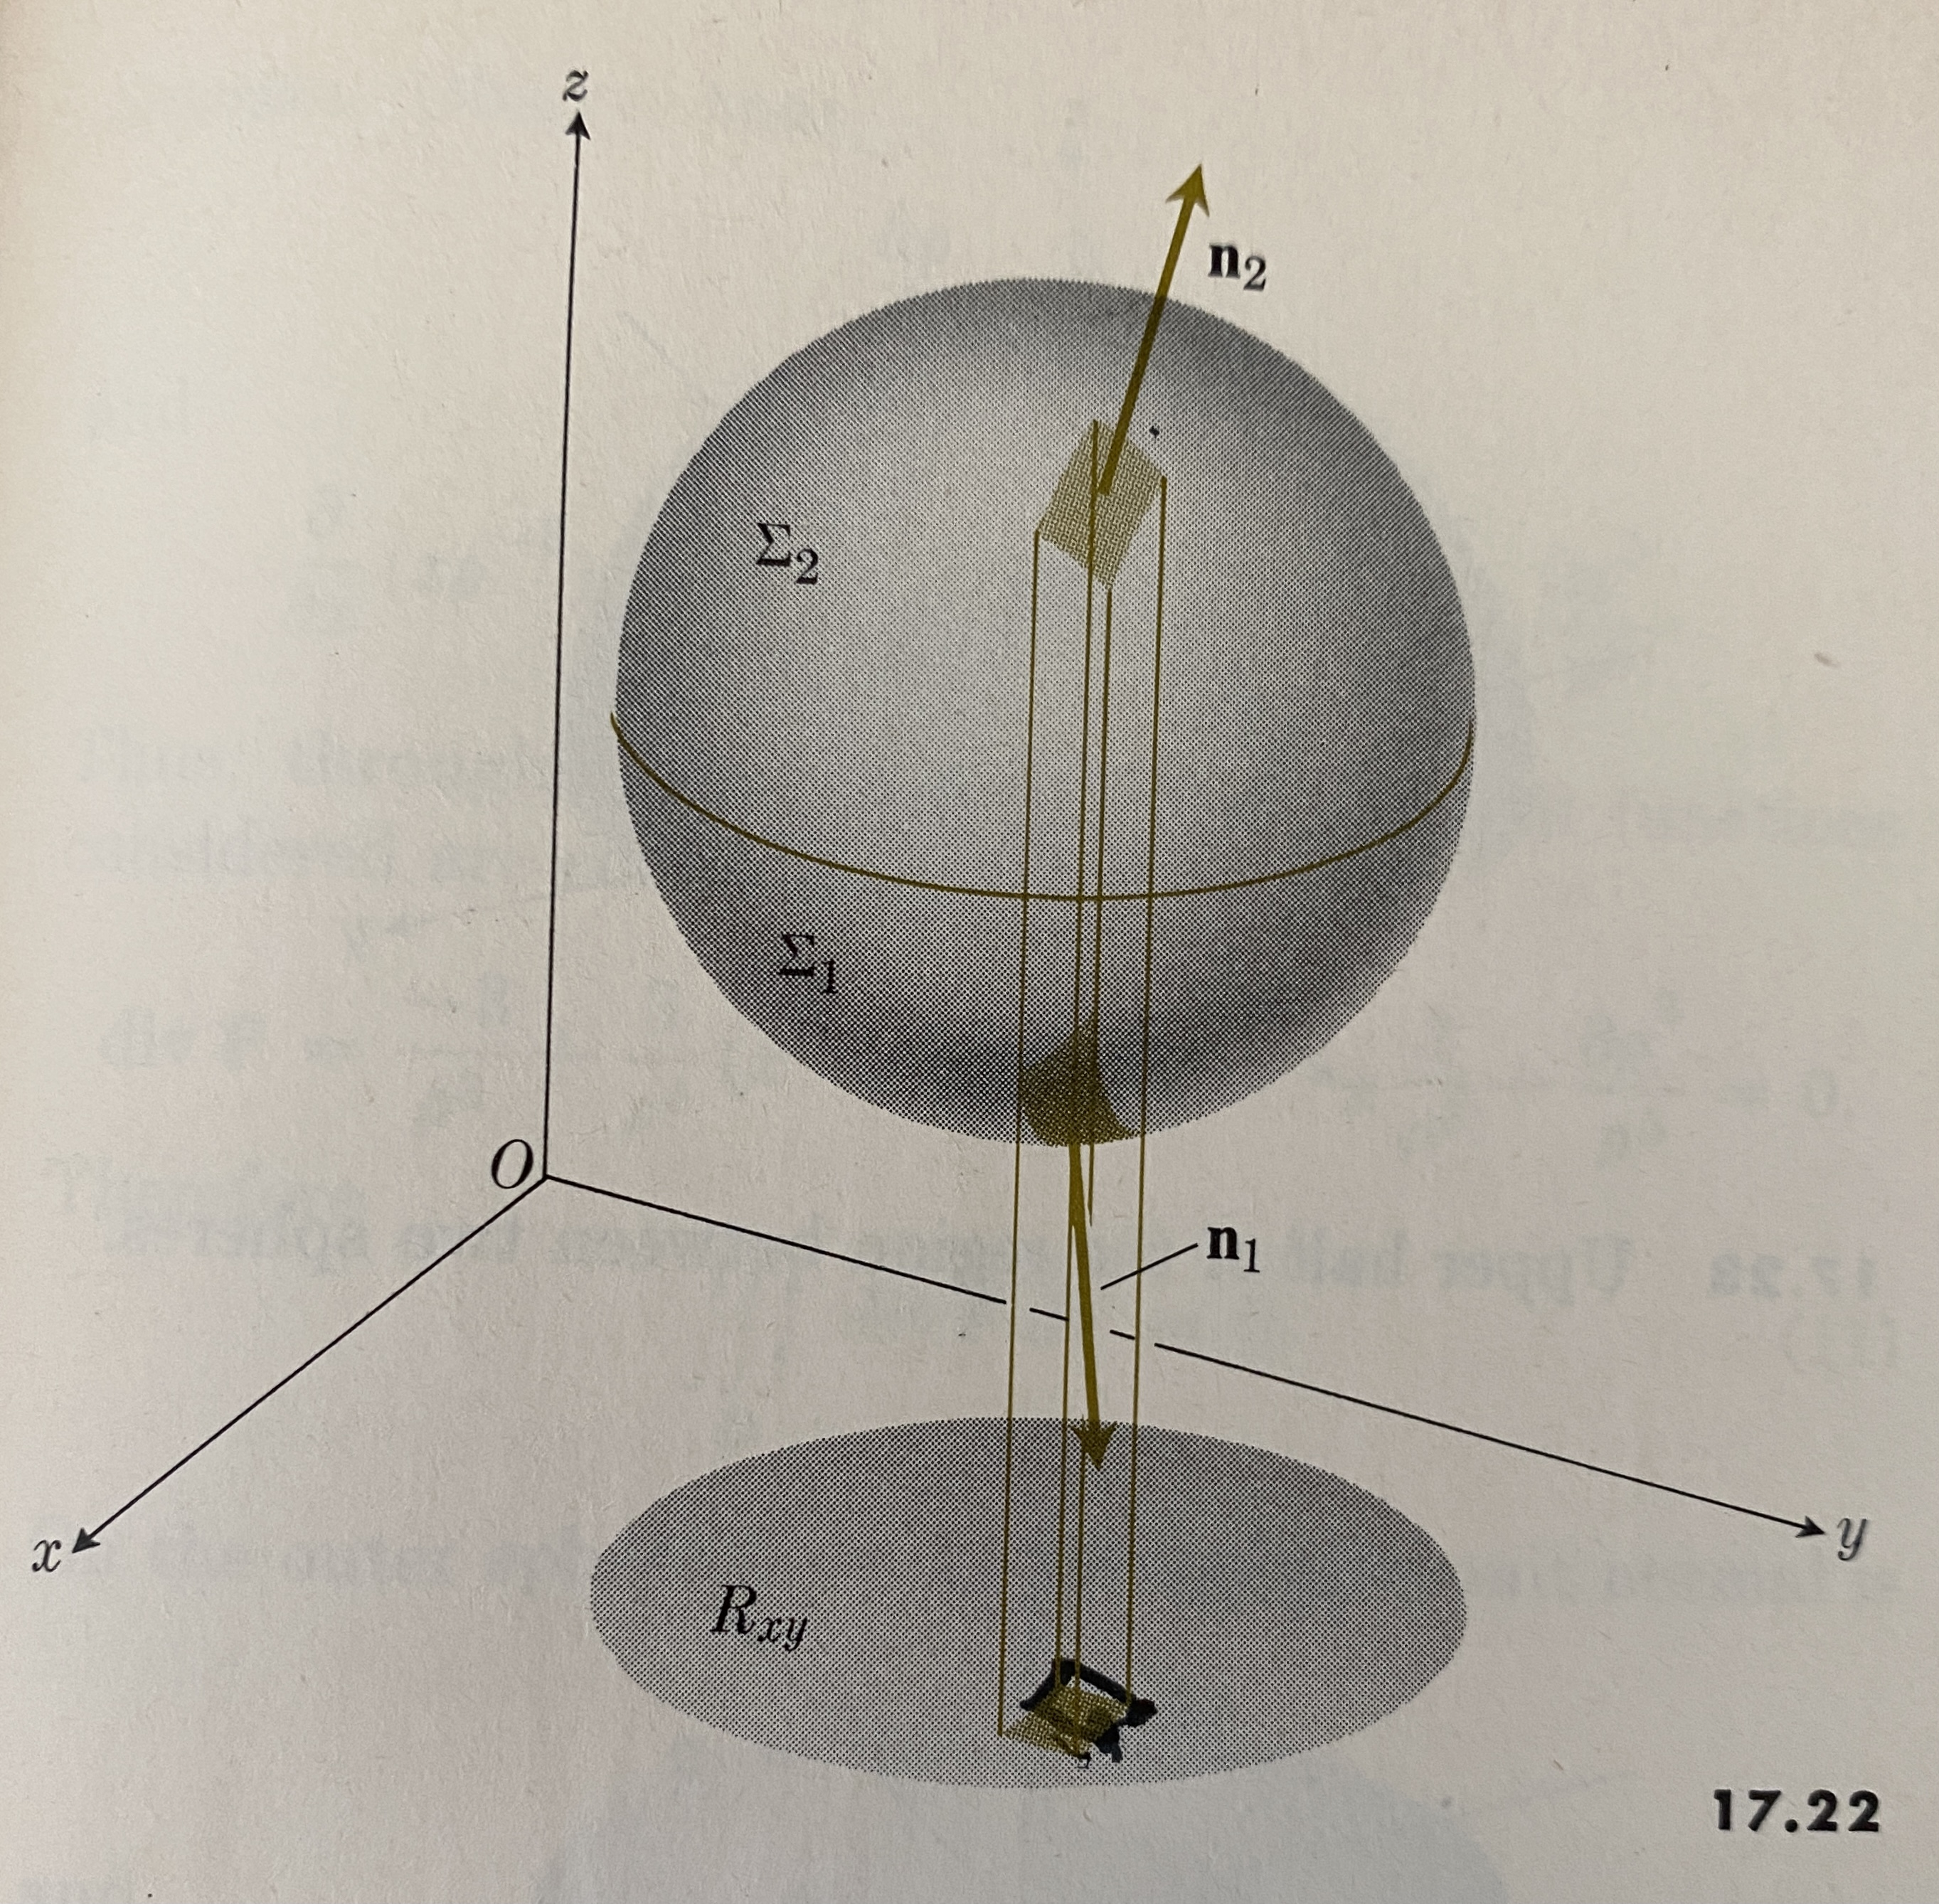
\includegraphics[width=0.4\linewidth]{ExtFiles/divergenceTheorem.jpg}
        \caption{Divergence theorem.}
        \label{fig:divergenceTheorem}
    \end{figure}
    \begin{itemize}
        \item We will not rigorously prove the divergence theorem, but we will justify $\iiint_D\pdv*{P}{z}\dd{x}\dd{y}\dd{z}=\iint_\Sigma P\cos\gamma\dd{\sigma}$.
        \item From Figure \ref{fig:divergenceTheorem}, we can see that the outer normal on $\Sigma_2$ has a positive $\mathbf{k}$-component, and so $\cos\gamma_2\dd{\sigma_2}=\dd{x}\dd{y}$.
        \item On the other hand, the outer normal on $\Sigma_1$ has a negative $\mathbf{k}$-component, so $\cos\gamma_1\dd{\sigma_1}=-\dd{x}\dd{y}$.
        \item Therefore,
        \begin{align*}
            \iint_\Sigma P\cos\gamma\dd{\sigma} &= \iint_{\Sigma_2}P_2\cos\gamma_2\dd{\sigma_2}+\iint_{\Sigma_1}P_1\cos\gamma_1\dd{\sigma_1}\\
            &= \iint_{R_{xy}}P(x,y,z_2)\dd{x}\dd{y}-\iint_{R_{xy}}P(x,y,z_1)\dd{x}\dd{y}\\
            &= \iint_{R_{xy}}[P(x,y,z_2)-P(x,y,z_1)]\dd{x}\dd{y}\\
            &= \iint_{R_{xy}}\int_{z_1}^{z_2}\left[ \pdv{P}{z}\dd{z} \right]\dd{x}\dd{y}\\
            &= \iiint_D\pdv{P}{z}\dd{x}\dd{y}\dd{z}
        \end{align*}
    \end{itemize}
    \item \dq{Verify [the divergence theorem] for the sphere $x^2+y^2+z^2=a^2$ if $\mathbf{F}=\mathbf{i}x+\mathbf{j}y+\mathbf{k}z$}{607}
    \begin{itemize}
        \item We will take this one piece at a time and then assemble all the pieces. We do this for both integrals in the divergence theorem.
        \item Left integral:
        \begin{itemize}
            \item First off,
            \begin{equation*}
                \text{div}\,\mathbf{F} = \pdv{x}{x}+\pdv{y}{y}+\pdv{z}{z} = 3
            \end{equation*}
            \item Therefore,
            \begin{equation*}
                \iiint_D\text{div}\,\mathbf{F}\dd{V} = \iiint_D3\dd{V} = 3\iiint_D\dd{V} = 3\left( \frac{4}{3}\pi a^3 \right) = 4\pi a^3
            \end{equation*}
        \end{itemize}
        \item Right integral:
        \begin{itemize}
            \item To define $\mathbf{n}$, we use the fact that $\mathbf{n}=\pm\nabla f/|\nabla f|$ where $f(x,y,z)=x^2+y^2+z^2-a^2$, meaning that the outer unit normal is
            \begin{equation*}
                \mathbf{n} = \frac{2x\mathbf{i}+2y\mathbf{j}+2z\mathbf{k}}{\sqrt{(2x)^2+(2y)^2+(2z)^2}} = \frac{x\mathbf{i}+y\mathbf{j}+z\mathbf{k}}{a}
            \end{equation*}
            \item It follows that
            \begin{equation*}
                \mathbf{F}\cdot\dd{\bm{\sigma}} = \frac{x^2+y^2+z^2}{a}\dd{\sigma} = \frac{a^2}{a}\dd{\sigma} = a\dd{\sigma}
            \end{equation*}
            \item Therefore,
            \begin{equation*}
                \iint_\Sigma\mathbf{F}\cdot\dd{\bm{\sigma}} = \iint_\Sigma a\dd{\sigma} = a(4\pi a^2) = 4\pi a^3
            \end{equation*}
        \end{itemize}
        \item Clearly, the two integrals are equal, as desired.
    \end{itemize}
    \item As with Green's theorem, the divergence theorem can be extended to more complex regions, as long as those regions can be split up into a finite number of simple regions of the type originally discussed.
    \item \textcite{bib:Thomas} proves that the divergence of the velocity of an incompressible fluid is zero in a region where there are no sources or sinks.
\end{itemize}



\section{Stokes's Theorem}
\begin{itemize}
    \item The following is a formal statement of \textbf{Stokes's theorem}.
    \begin{thm}[Stokes's theorem]
        Let $\Sigma$ be a smooth, simply connected, orientable surface bounded by a simple closed curve $C$. Let $\mathbf{F}=\mathbf{i}M+\mathbf{j}N+\mathbf{k}P$, where $M,N,P$ are continuous functions of $(x,y,z)$, together with their first-order partial derivatives throughout a region $D$ containing $\Sigma$ and $C$ in its interior. Let $\mathbf{n}$ be a positive unit vector normal to $\Sigma$, and let the positive direction around $C$ be the one induced by the positive orientation of $\Sigma$. Then
        \begin{equation*}
            \oint_C\mathbf{F}\cdot\dd{\mathbf{R}} = \iint_\Sigma\text{curl}\,\mathbf{F}\cdot\dd{\bm{\sigma}}
        \end{equation*}
        where $\dd{\mathbf{R}}=\mathbf{i}\dd{x}+\mathbf{j}\dd{y}+\mathbf{k}\dd{z}=\mathbf{T}\dd{s}$ and $\dd{\bm{\sigma}}=\mathbf{n}\dd{\sigma}=(\mathbf{i}\cos\alpha+\mathbf{j}\cos\beta+\mathbf{k}\cos\gamma)\dd{\sigma}$.
    \end{thm}
    \begin{itemize}
        \item \textcite{bib:Thomas} proves Stokes's theorem from Green's theorem for a polyhedral surface consisting of a finite number of plane regions, much the same way he built up larger surfaces from Green's theorem earlier on.
        \item A rigorous proof of Stokes's theorem for more general surfaces is beyond the level of an intro calculus course. More intuitively, we can think about taking the limit of a finite construction for more and more subdivision of a general surface.
    \end{itemize}
    \item \textbf{Orientable} (surface): A surface $\Sigma$ such that it is possible to consistently assign a unique direction, called positive, at each point of $\Sigma$. As we move the normal over $\Sigma$ without touching its boundary, the direction cosines of the unit vector $\mathbf{n}$ should vary continuously. Also, when we return to the starting position, $\mathbf{n}$ should return to its original direction.
    \begin{itemize}
        \item Recall that M\"{o}bius strips are non-orientable surfaces.
    \end{itemize}
    \item Defining the positive direction around $C$ consistently with the positive direction on $\Sigma$.
    \begin{figure}[h!]
        \centering
        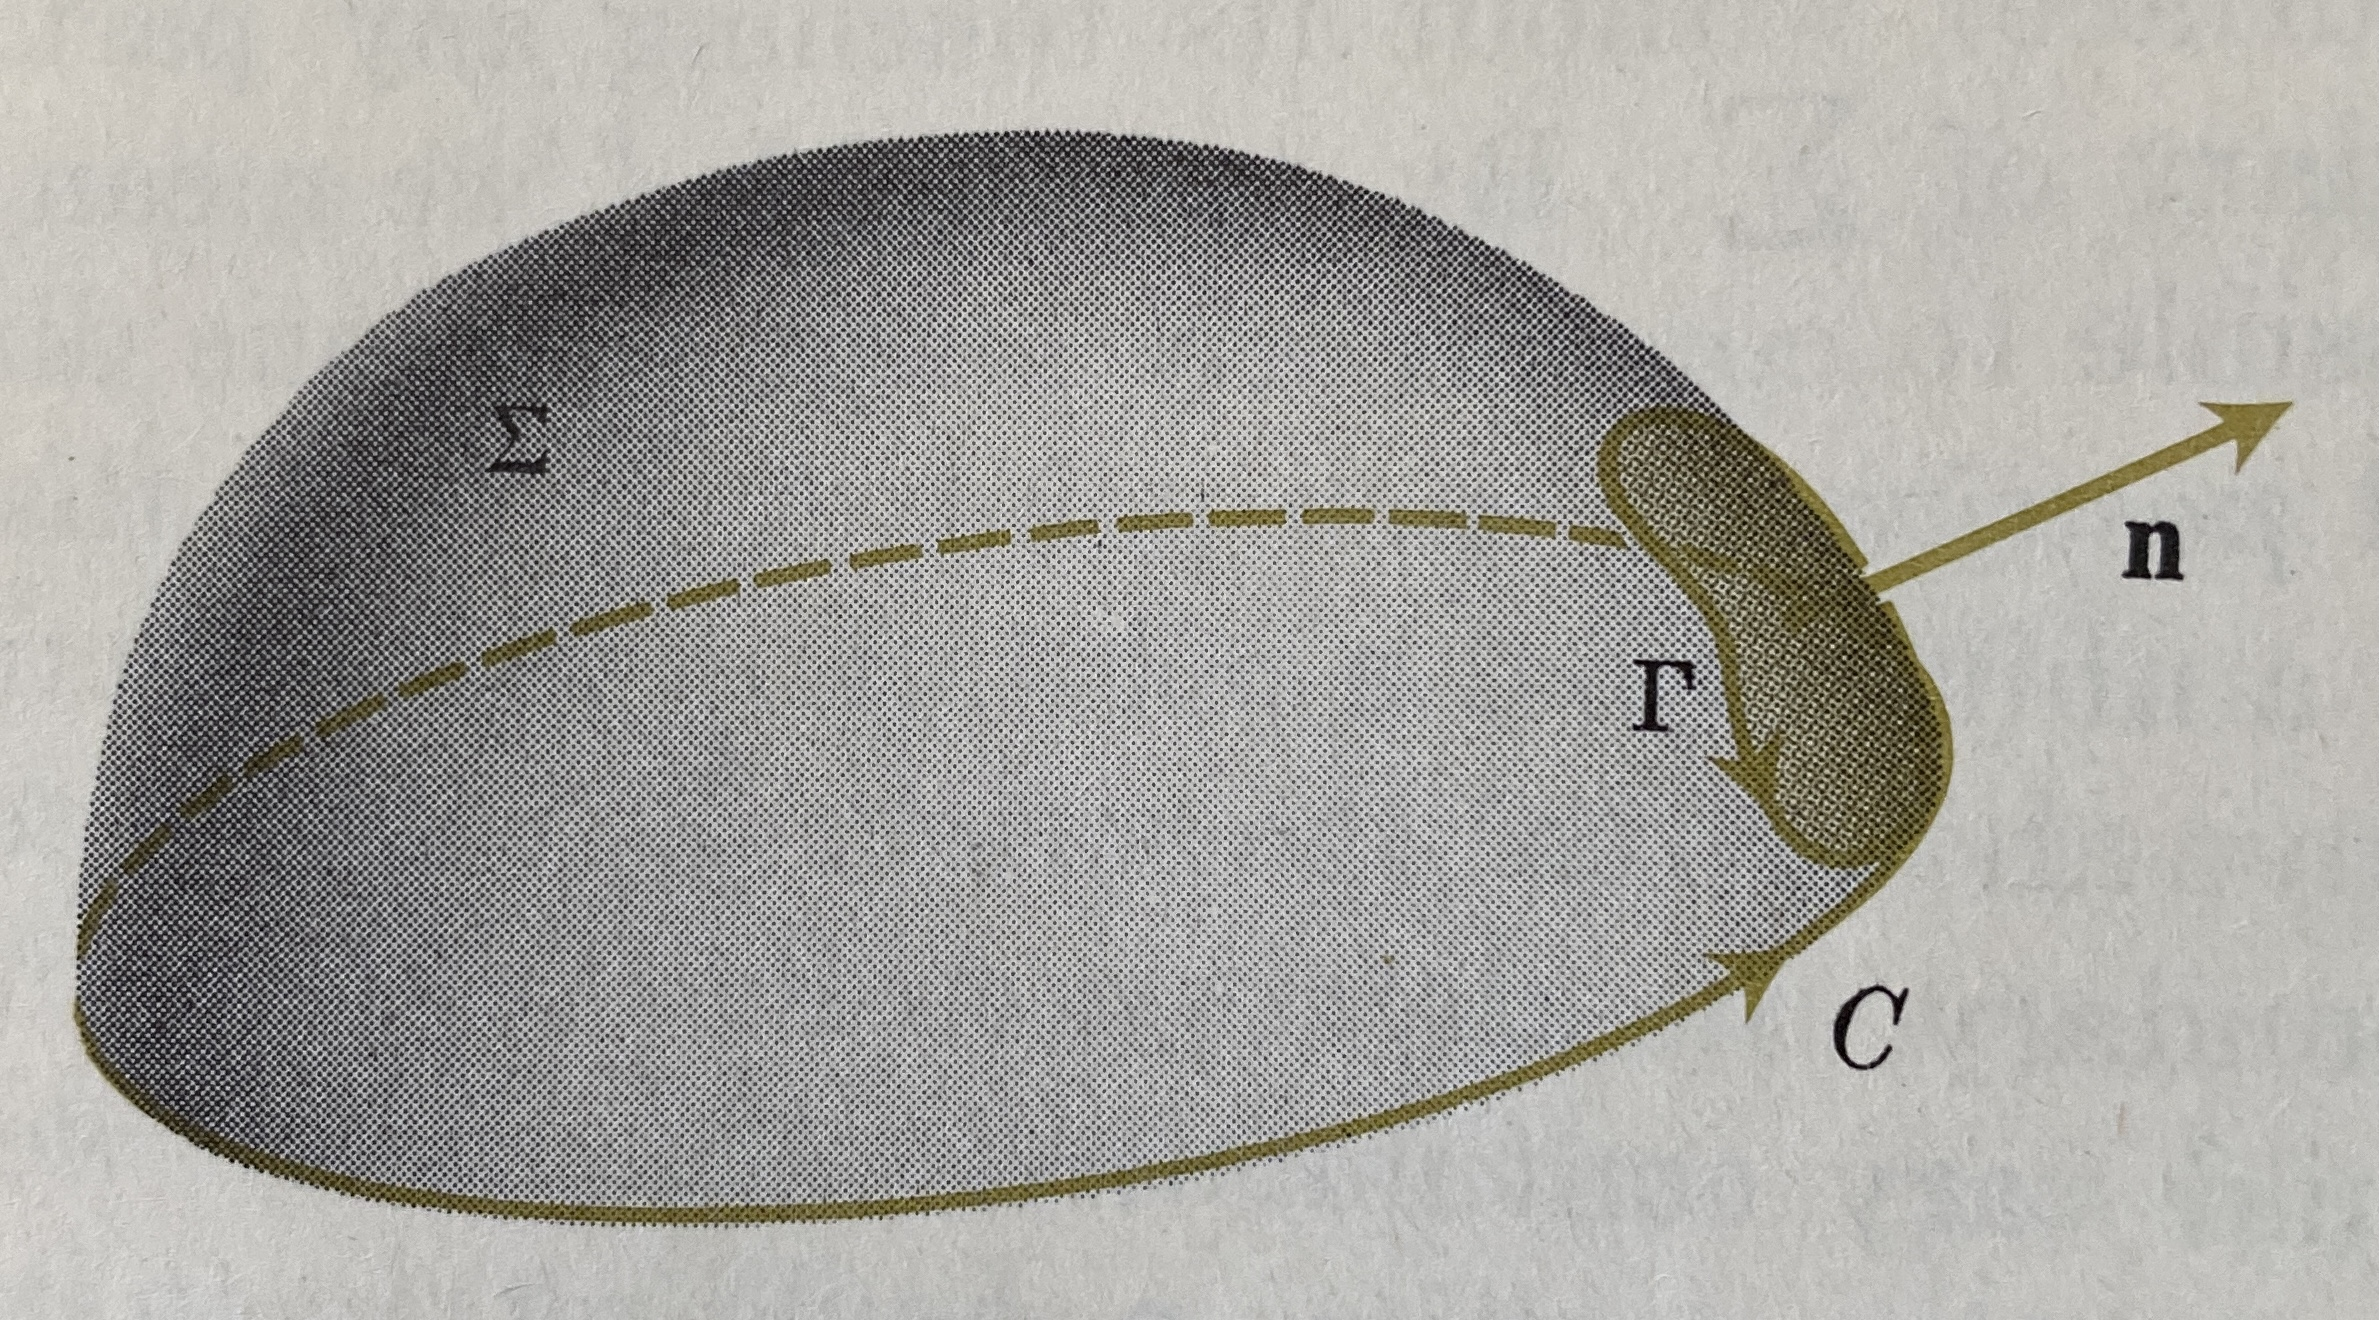
\includegraphics[width=0.3\linewidth]{ExtFiles/orientingSurface-Boundary.jpg}
        \caption{Orienting a surface and its boundary consistently.}
        \label{fig:orientingSurface-Boundary}
    \end{figure}
    \begin{itemize}
        \item \dq{Imagine a simple closed curve $\Gamma$ on $\Sigma$, near the boundary $C$, and let $\mathbf{n}$ be normal to $\sigma$ at some point inside $\Gamma$. We then assign to $\Gamma$ a positive direction, the counterclockwise direction as viewed by an observer who is at the end of $\mathbf{n}$ and looking down. (Note that such a direction keeps the interior of $\Gamma$ on the observer's left as he progresses around $\Gamma$. We could equally well have specified $\mathbf{n}$'s direction by this condition.) Now we move $\Gamma$ about $\Sigma$ until it touches and is tangent to $C$. The direction of the positive tangent to $\Gamma$ at this point of common tangency we shall take to be the positive direction along $C$}{612}
        \item Note that it is a consequence of the orientability of $\Sigma$ that a consistent assignment of positive direction along $C$ is induced by this process (it would not hold for a M\"{o}bius strip, for example).
    \end{itemize}
    \item \dq{Let $S$ be the portion of the paraboloid $z=4-x^2-y^2$ that lies above the plane $z=0$. Let $C$ be their curve of intersection, and let $\mathbf{F}=\mathbf{i}(z-y)+\mathbf{j}(z+x)-\mathbf{k}(x+y)$. Compute $\oint_C\mathbf{F}\cdot\dd{\mathbf{R}}$ and $\iint_S\text{curl}\,\mathbf{F}\cdot\dd{\bm{\sigma}}$ and compare}{614}
    \begin{itemize}
        \item Naturally, $C$ is defined by $z=0=4-x^2+y^2$, or $x^2+y^2=4$.
        \item With the substitutions $x=2\cos\theta$, $y=2\sin\theta$, and $z=0$, we get the following.
        \begin{align*}
            \oint_C\mathbf{F}\cdot\dd{\mathbf{R}} &= \oint_C(z-y)\dd{x}+(z+x)\dd{y}-(x+y)\dd{z}\\
            &= \int_0^{2\pi}(0-2\sin\theta)(-2\sin\theta\dd{\theta})+(0+2\cos\theta)(2\cos\theta\dd{\theta})+(2\cos\theta+2\sin\theta)(0)\\
            &= \int_0^{2\pi}4(\sin^2\theta+\cos^2\theta)\dd{\theta}\\
            &= 4\int_0^{2\pi}\dd{\theta}\\
            &= 8\pi
        \end{align*}
        \begin{itemize}
            \item Note that we can also evaluate $\oint_C\mathbf{F}\cdot\dd{\mathbf{R}}$ more directly with
            \begin{equation*}
                \begin{split}
                    \oint_C\mathbf{F}\cdot\dd{\mathbf{R}} &= \left[ \int_2^{-2}\left( 0-\sqrt{4-x^2} \right)\dd{x}+\int_{-2}^2\left( 0-\left( -\sqrt{4-x^2} \right) \right)\dd{x} \right]\\
                    &\qquad+\left[ \int_2^{-2}\left( 0-\sqrt{4-y^2} \right)\dd{y}+\int_{-2}^2\left( 0-\left( -\sqrt{4-y^2} \right) \right)\dd{y} \right]
                \end{split}
            \end{equation*}
        \end{itemize}
        \item As to the other integral, we'll do some setup first.
        \item First off, we have
        \begin{align*}
            \text{curl}\,\mathbf{F} &=
            \begin{vmatrix}
                \mathbf{i} & \mathbf{j} & \mathbf{k}\\
                \pdv{x} & \pdv{y} & \pdv{z}\\
                z-y & z+x & -x-y\\
            \end{vmatrix}\\
            &= -2\mathbf{i}+2\mathbf{j}+2\mathbf{k}
        \end{align*}
        \item Next up, if $f(x,y,z)=z-4+x^2+y^2$, we have
        \begin{align*}
            \mathbf{n} &= \frac{\nabla f}{|\nabla f|}\\
            &= \frac{2x\mathbf{i}+2y\mathbf{j}+\mathbf{k}}{\sqrt{4x^2+4y^2+1}}
        \end{align*}
        \item To evaluate this surface integral, we'll project it onto the $xy$-plane. Its shadow is $x^2+y^2\leq 4$.
        \item And to account for this change of domain, we must use
        \begin{align*}
            \dd{\sigma} &= \sqrt{\left( \pdv{z}{x} \right)^2+\left( \pdv{z}{y} \right)^2+1}\dd{x}\dd{y}\\
            &= \sqrt{4x^2+4y^2+1}\dd{x}\dd{y}
        \end{align*}
        \item Putting everything together, we have
        \begin{align*}
            \iint_S\text{curl}\,\mathbf{F}\cdot\mathbf{n}\dd{\sigma} &= \iint_{x^2+y^2\leq 4}(-2\mathbf{i}+2\mathbf{j}+2\mathbf{k})\cdot\frac{2x\mathbf{i}+2y\mathbf{j}+\mathbf{k}}{\sqrt{4x^2+4y^2+1}}\sqrt{4x^2+4y^2+1}\dd{x}\dd{y}\\
            &= \iint_{x^2+y^2\leq 4}(-4x+4y+2)\dd{x}\dd{y}\\
            &= \iint_{x^2+y^2\leq 4}2\dd{x}\dd{y}\\
            &= 2(\pi\cdot 2^2)\\
            &= 8\pi
        \end{align*}
        \begin{itemize}
            \item Note that we can remove $-4x+4y$ from the integrand because odd powers of $x$ or $y$ integrate to 0 over the interior of the circle.
        \end{itemize}
    \end{itemize}
    \item Stokes's theorem can also be extended to a surface with finitely many holes in a manner analogously to how we did so with Green's theorem.
    \item Note that Stokes's theorem interprets curl as equating the circulation of fluid around the closed curve $C$ with the flus of the curl though the surface spanning $C$.
\end{itemize}




\end{document}